\documentclass{article}
\usepackage{ifxetex}
\ifxetex
  \usepackage{fontspec}
\else
  \usepackage[T1]{fontenc}
  \usepackage[utf8]{inputenc}
  \usepackage{lmodern}
\fi
\title{Problem Set 8}
\author{%
    Ishan Pranav
\\  MATH-UA 120 Discrete Mathematics
}
\date{due December 8, 2023}
\usepackage[headings=runin-fixed-nr]{exsheets}
\makeatletter
    \newcommand{\stepenumdepth}{\advance\@enumdepth\@ne}
\makeatother
\SetupExSheets{
    question/pre-body-hook=\stepenumdepth,
    solution/pre-body-hook=\stepenumdepth,
}
\DeclareInstance{exsheets-heading}{runin-nn-np}{default}{
    runin = true,
    title-post-code = .\space,
    join = {
        main[r,vc]title[l,vc](0pt,0pt);
    }
}
\newif\ifshowsolutions
\showsolutionstrue
\ifshowsolutions
    \SetupExSheets{
        question/pre-hook=\itshape,
        solution/headings=runin-nn-np,
        solution/print=true,
        solution/name=Answer
    }%
    \makeatletter%
    \pretocmd{\@title}{Answers to }%
    \makeatother%
\else
    \SetupExSheets{solution/print=false}
\fi

% Bug workaround: http://tex.stackexchange.com/a/146536/1402
%\newenvironment{exercise}{}{}
\RenewQuSolPair{question}{solution}
%\let\answer\solution
%\let\endanswer\endsolution
\usepackage{manfnt}
\newcommand{\danger}{\marginpar[\hfill\dbend]{\dbend\hfill}}
\newcommand{\Z}{\mathbb{Z}}
\newcommand{\N}{\mathbb{N}}
\newcommand{\modulo}{\text{ mod }}
\newcommand{\divisor}{\text{ div }}
\usepackage{tikz}
\tikzstyle{vertex}=[circle,draw,fill=none,inner sep=0pt,outer sep=0pt, minimum width=1ex]
\tikzstyle{edge}=[draw,thick]
\usepackage{multirow, multicol}
\usepackage{amsmath, amsthm, amssymb}
\usepackage{amsfonts}
\usepackage{siunitx}
\DeclareSIUnit\pound{lb}
\usepackage{hyperref}
\newtheorem*{theorem}{Theorem}
\theoremstyle{definition}
\newtheorem*{definition}{Definition}
\newenvironment{note}{\noindent\emph{Note}.}{}
\begin{document}
\maketitle
These are to be written up and turned in to Gradescope.\\

\ifshowsolutions
    \SetupExSheets{solution/print=true}
\else
    \danger
 \underline{ \LaTeX  Instructions:}  You can view the source (\texttt{.tex}) file to get some more examples of \LaTeX{} code.  I have commented the source file in places where new \LaTeX{} constructions are used.
  
  Remember to change \verb|\showsolutionsfalse| to \verb|\showsolutionstrue|
    in the document's preamble 
    (between \verb|\documentclass{article}| and \verb|\begin{document}|)
\fi
\section*{Assigned Problems}
\begin{question}
    \begin{enumerate}
        \item Find $d = \gcd(29341,1739)$, and integers $x$ and $y$ such that $29341x + 1739y = d$.
        \item Prove that 7 cannot be expressed as an integral linear combination of 29341 and 1739.
    \end{enumerate}
\end{question}
\begin{solution}
Let $d=\gcd(29341,1739)$. Observe
\begin{align*}
d
&=\gcd(29341,1739)\\
&=\gcd(1739,29341 \modulo 1739)&\text{(note }29341-16\cdot 1739=1517\text{)}\\
&=\gcd(1517,1739 \modulo 1517)&\text{(note }1739-1\cdot 1517=222\text{)}\\
&=\gcd(222,1739 \modulo 222)&\text{(note }1517-6\cdot 222=185\text{)}\\
&=\gcd(185,222 \modulo 185)&\text{(note }222-1\cdot 185=37\text{)}\\
&=\gcd(37,185 \modulo 37)&\text{(note }185-5\cdot 37=0\text{)}\\
&=37.
\end{align*}
Consider $37=29341x+1739y$. Observe
\begin{align*}
0\cdot 29341+1\cdot 1739&=1739\\
1\cdot 29341-16\cdot 1739&=1517\\
-1\cdot 29341+17\cdot 1739&=222\\
7\cdot 29341-118\cdot 1739&=185\\
-8\cdot 29341+135\cdot 1739&=37\\
29341x+1739y&=37.
\end{align*}
Thus $x=-8$ and $y=135$.
\end{solution}
\begin{question}
    \begin{enumerate}
        \item Disprove: There exist integers $a$ and $b$ such that $a+b=100$ and $\gcd(a, b)=8$.
        \item Prove: There exist infinitely many pairs of integers $(a,b)$ such that $a+b=87$ and $\gcd(a, b)=3$.
    \end{enumerate}
\end{question}
% Student: put your answer between the next two lines.
\begin{solution}
\end{solution}

\begin{question}
    \begin{enumerate}
        \item Let $a, b, c\in \Z$ such that $a$ and $b$ are relatively prime. Prove that if $a\mid c$ and $b\mid c$, then $(ab)\mid c$.
        \item Explain why part (a) is false if $a$ and $b$ are not relatively prime.
    \end{enumerate}
\end{question}
% Student: put your answer between the next two lines.
\begin{solution}
\end{solution}

\begin{question} 
 Consider the following graph $G$.
     \begin{center}
    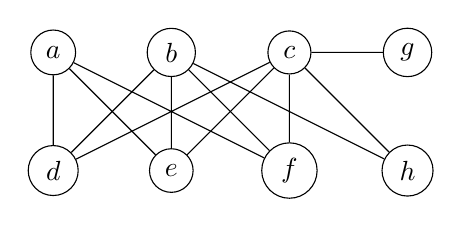
\begin{tikzpicture}[
        every node/.append style={draw,circle}
    ]
        \node (A) at (-1.5, 0) {$a$};
        \node (B) at (0, 0)    {$b$};
        \node (C) at (1.5, 0)  {$c$};
        \node (D) at (-1.5, -1.5) {$d$};
        \node (E) at (0, -1.5)   {$e$};
        \node (F) at (1.5, -1.5) {$f$};
        \node (G) at (3, 0)   {$g$};
        \node (H) at (3, -1.5) {$h$};
        \draw (A) -- (D) -- (C) -- (F) -- (A);
        \draw (A) -- (E) -- (C);
        \draw (D) -- (B) -- (F);
        \draw (G) -- (C) -- (H) -- (B) -- (E);
    \end{tikzpicture}
    \end{center}
    
\begin{enumerate}
	\item Write out the ordered pair $G=(V, E)$.
	\item What is the order of $G$?
	\item What is the size of $G$?
	\item What is $N(b)$?
	\item What is $d_G(c)$?
	\item What is $\Delta(G)$?
	\item What is $\delta(G)$?
	\item What elements are the vertex $a$ adjacent to?
	\item What elements are the vertex $f$ incident with?
	\item Is $G$ regular? Briefly explain why or why not.
	\end{enumerate}
\end{question}
% Student: put your answer between the next two lines.
\begin{solution}
\end{solution}

\begin{question}
     Let $G=(V,E)$ be a graph. Prove by induction: 
\begin{quote}
The sum of the degrees of the vertices in $G$ is twice the number of edges.
\end{quote}	
\end{question}
% Student: put your answer between the next two lines.
\begin{solution}
\end{solution}









\end{document}